%%%%%%%%%%%%%%%%%%%%%%%%%%%%%%%%%%%%%%%%%
% Journal Article
% LaTeX Template
% Version 1.4 (15/5/16)
%
% This template has been downloaded from:
% http://www.LaTeXTemplates.com
%
% Original author:
% Frits Wenneker (http://www.howtotex.com) with extensive modifications by
% Vel (vel@LaTeXTemplates.com)
%
% License:
% CC BY-NC-SA 3.0 (http://creativecommons.org/licenses/by-nc-sa/3.0/)
%
%%%%%%%%%%%%%%%%%%%%%%%%%%%%%%%%%%%%%%%%%

%----------------------------------------------------------------------------------------
%	PACKAGES AND OTHER DOCUMENT CONFIGURATIONS
%----------------------------------------------------------------------------------------

\documentclass[twoside]{article}
\usepackage{blindtext} % Package to generate dummy text throughout this template

\usepackage[sc]{mathpazo} % Use the Palatino font
\usepackage[T1]{fontenc} % Use 8-bit encoding that has 256 glyphs
\linespread{1.05} % Line spacing - Palatino needs more space between lines
\usepackage{microtype} % Slightly tweak font spacing for aesthetics
\usepackage{amsmath}
\usepackage{listings}
\usepackage{mathtools}
\usepackage[english]{babel} % Language hyphenation and typographical rules

\usepackage[hmarginratio=1:1,top=25mm,columnsep=20pt]{geometry} % Document margins
\usepackage[hang, small,labelfont=bf,up,textfont=it,up]{caption} % Custom captions under/above floats in tables or figures
\usepackage{booktabs} % Horizontal rules in tables

\usepackage{lettrine} % The lettrine is the first enlarged letter at the beginning of the text

\usepackage{enumitem} % Customized lists
\setlist[itemize]{noitemsep} % Make itemize lists more compact

\usepackage{abstract} % Allows abstract customization
\renewcommand{\abstractnamefont}{\normalfont\bfseries} % Set the "Abstract" text to bold
\renewcommand{\abstracttextfont}{\normalfont\small\itshape} % Set the abstract itself to small italic text

\usepackage{titlesec} % Allows customization of titles
\renewcommand\thesection{\Roman{section}} % Roman numerals for the sections
\renewcommand\thesubsection{\roman{subsection}} % roman numerals for subsections
\titleformat{\section}[block]{\large\scshape\centering}{\thesection.}{1em}{} % Change the look of the section titles
\titleformat{\subsection}[block]{\large}{\thesubsection.}{1em}{} % Change the look of the section titles

\usepackage{fancyhdr} % Headers and footers
\pagestyle{fancy} % All pages have headers and footers
\fancyhead{} % Blank out the default header
\fancyfoot{} % Blank out the default footer
% \fancyhead[C]{Running title $\bullet$ May 2016 $\bullet$ Vol. XXI, No. 1} % Custom header text

% \fancyfoot[C]{\shortstack{\thepage \\ \\ \small Thatcher Imaging LLC | BEARE MEDIA (PTY) LTD | Not for Redistribution}}
\fancyfoot[C]{\thepage}

\usepackage{titling} % Customizing the title section

\usepackage{hyperref} % For hyperlinks in the PDF

%----------------------------------------------------------------------------------------
%	TITLE SECTION
%----------------------------------------------------------------------------------------

\setlength{\droptitle}{-4\baselineskip} % Move the title up

\pretitle{\begin{center}\Huge\bfseries} % Article title formatting
\posttitle{\end{center}} % Article title closing formatting
\title{Guidelines for Camera Matching} % Article title
\author{%
    \textsc{Thatcher Freeman} \\[1ex] % Your name
    % \normalsize \href{mailto:me@thatcherfreeman.com}{me@thatcherfreeman.com}
    \normalsize \href{https://github.com/thatcherfreeman}{github.com/thatcherfreeman}
}
\date{}%\today} % Leave empty to omit a date
\renewcommand{\maketitlehookd}{%
    \begin{abstract}
    \noindent Two cameras can be approximately matched by a 3x3 matrix, applied in the scene linear domain. The selection of this matrix is done by minimizing the error between the patches on a color chart shot with both cameras, under lighting representative of the intended shooting conditions. This document will explain how to best conduct the photography needed to perform this matching process.
    \end{abstract}
}

%----------------------------------------------------------------------------------------

\begin{document}

% Print the title
\maketitle
\thispagestyle{fancy}

%----------------------------------------------------------------------------------------
%	ARTICLE CONTENTS
%----------------------------------------------------------------------------------------
\tableofcontents
\newpage
\section{Prerequisites}
The camera match is generally dependent on the choice of lens, the lighting illuminant, codec, white balance setting, and sometimes the base ISO and exposure used. Select these such that they are representative of the intended shooting conditions. The more that the actual setup differs from the profiling setup, the less accurate the camera match will be. \\

It is also necessary to record with a log encoding which we can easily linearized (eg, supported by DaVinci Resolve or ACES or via a custom linearization profile). We have separate documentation for if your camera is not supported by these systems, and if you're unsure, feel free to reach out and we can help you profile the camera's log curve. \\

The above must be selected and used for each camera intended to be matched. \\

\section{Color Chart}

We recommend using a Calibrite ColorChecker Classic color chart (pictured in Figure \ref{chart_tips}). If using a different color chart, then select one that has a wide range of non-grey colors, including some skin tones. The ColorChecker Video chart is \textbf{NOT} recommended due to its low color diversity.


\begin{figure}[h]
    \centering
    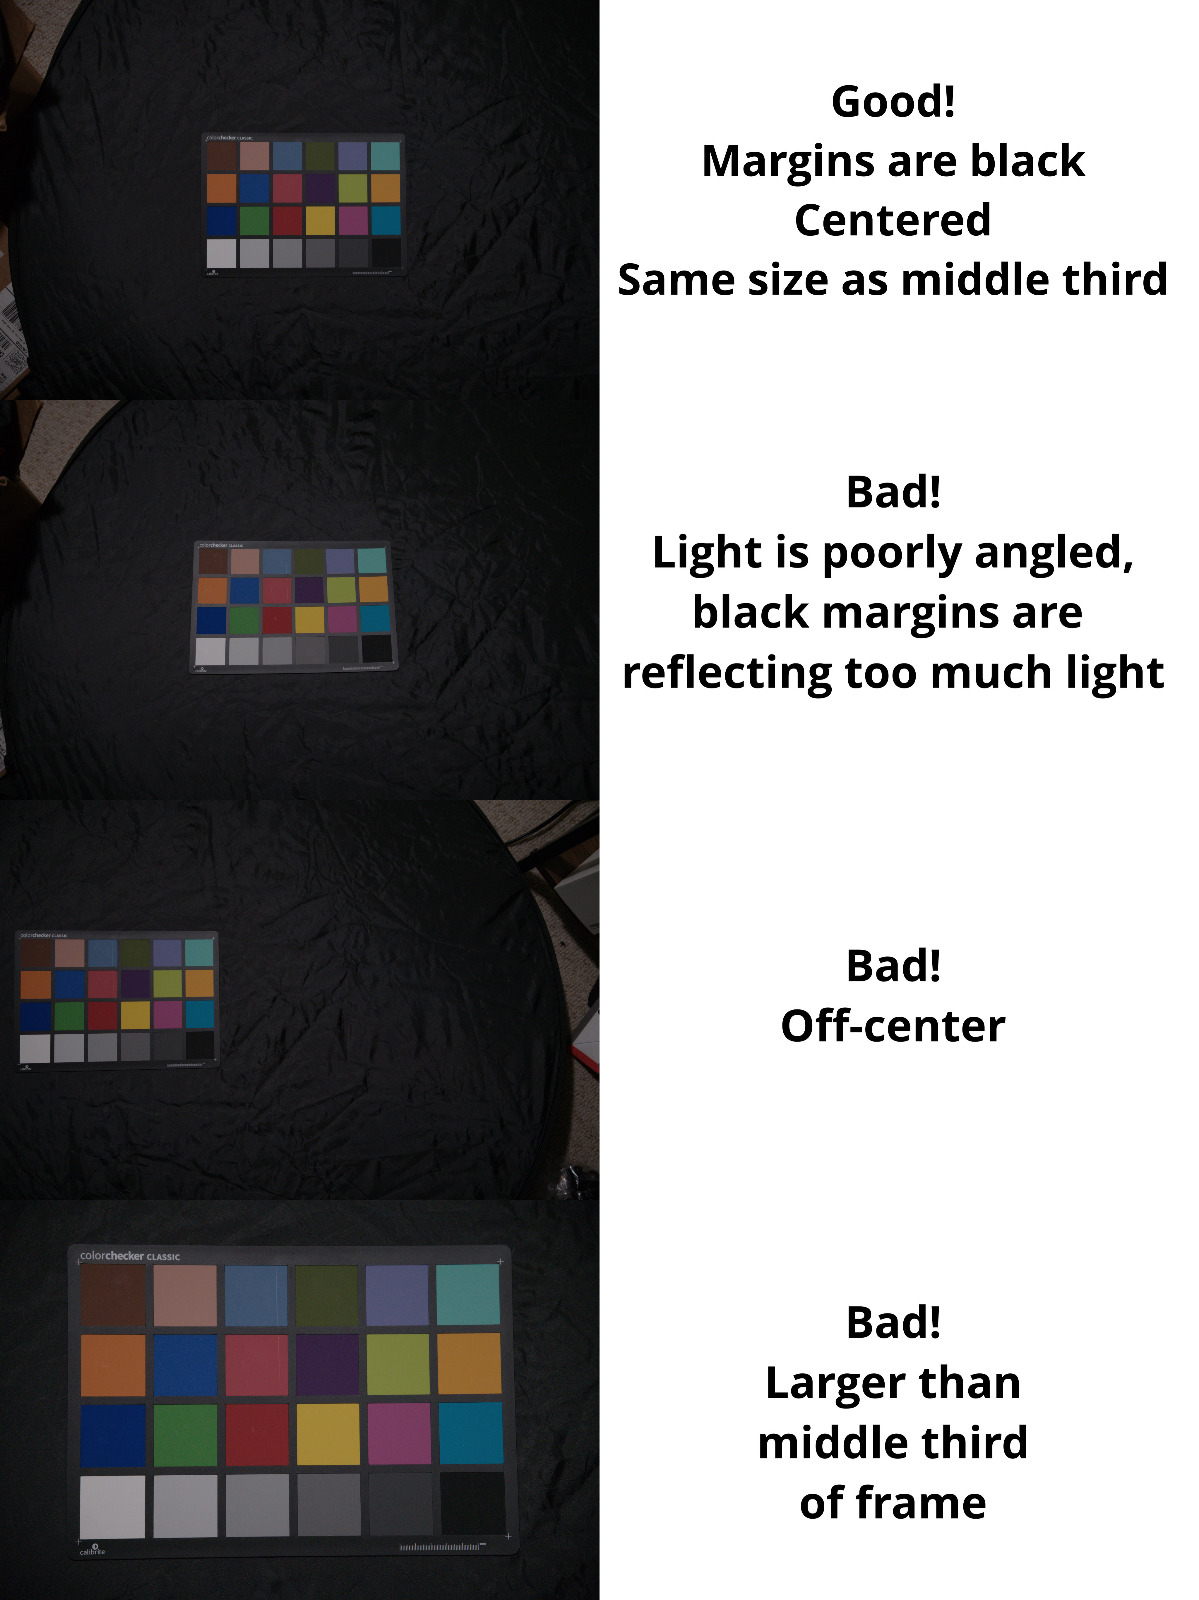
\includegraphics[scale=0.2]{images/Chart Tips.jpg}
    \caption{Composition and Chart Angle Guide}
    \label{chart_tips}
\end{figure}

\newpage
\section{Procedure}

Follow the below requirements with each camera to be matched. Each camera should be independently white balanced and their positions (and particularly their angle with respect to the chart) should be approximately matched. The quality of the color match is dependent on the degree to which this procedure is followed and to how similar these conditions are to the real production camera configuration and lighting.


\subsection{Requirements}
\begin{enumerate}
    \item \textbf{Angle the chart to control glare} - The light should be placed at such an angle to the color chart that the camera is not in-line with the primary reflection of the light in the color chart. IE if the color chart were a mirror, the light's reflection should not be visible to the camera. If the camera is normal to the test chart, putting the light at a 45 degree angle to the test chart would easily avoid this. See Figure \ref{chart_tips}
    \item \textbf{Even lighting on the color chart} - Place the light far from the test chart so that the light hitting the chart is uniform (place the light at least 4x the length of the long side of the test chart away).
    \item \textbf{Correct white balance} - The camera should be white balanced for this light source. If white balancing via Kelvins is to be used, choose the best Kelvin white balance for the light, for each camera. Alternatively, AWB off of a white card illuminated by your light source. If the camera is to be used with a single white balance for the entire production, just use that white balance.
    \item \textbf{Proper exposure} - Properly expose the color chart with a light meter. Ensure that no chip on the color chart is clipped, and make sure that it's not underexposed.
    \item \textbf{Color chart fills the middle third of the image} - This is a compromise between maximizing the number of pixels we can sample for each color chip, and avoiding lens vignetting. Fill the middle rule of thirds box with the color chart.
    \item \textbf{Dark background material to control lens flaring} - We don't want there to be any bright spots in the background of the image that could result in lens flaring, as this would contaminate the chart colors.
    \item \textbf{Lens stopped down a couple stops} - By stopping down the lens, contrast and flare are typically improved. Pick an aperture in the range of f/4-f/8, if possible.
    \item \textbf{Lock off the tripod} - By keeping the chart and tripod stationary, this makes it easier for us to denoise the chart and extract its true colors
    \item \textbf{1-5s Duration} - It is only necessary to shoot the chart for between 1 and 5 seconds.
    \item \textbf{Do not obscure the color chart} - Do not let shadows or fingers or clamps cover any part of the color chips on the chart.
\end{enumerate}

\newpage
\section{Edge Cases}
\subsection{Rapidly Changing Lighting Conditions}
If the test has to be shot under rapidly variable lighting conditions, then it is advisable to put your cameras next to each other and record the chart simultaneously.

\subsection{Colored Filtration}
If using filters that have a strong color cast, it may be useful to build the camera match for a single camera under each filter in question so we can match them to the hero setup. This is simply a matter of following the procedure with one camera but for each filter or lens.


\end{document}